\documentclass[twocolumn,a4paper]{ctexart}
\usepackage[UTF8,scheme=plain]{ctex}

\usepackage{cite}
\usepackage{amsmath,amssymb,amsfonts}
\usepackage{graphicx}
\usepackage{textcomp}
\usepackage{xcolor}
\usepackage{booktabs}
\usepackage{url}
\usepackage[margin=1.9cm]{geometry}
\usepackage{abstract}
\graphicspath{{figures/}}

\title{\bfseries A Self-Evolving Reinforcement Learning System\\ for Agentic Large Language Models}
\author{Hao Sun\\[2pt] \normalsize School of Smart Governance, Renmin University of China}
\date{}

\begin{document}

\twocolumn[
\maketitle
\begin{onecolabstract}
\noindent\textbf{Abstract}\quad Large language model (LLM) agents accomplish tasks through multi-step tool use in real environments such as code sandboxes and file systems, where reinforcement learning (RL) has become the dominant approach for continuous improvement. However, RL for interactive agents faces a fundamental bottleneck: both training data and trustworthy rewards are difficult to obtain at scale through human effort. Real user data accumulates slowly with narrow coverage, and rewards that rely solely on agent self-reports invite reward hacking, where the model learns to falsely claim task completion. We present a \emph{self-evolving} RL system for agentic LLMs that enables agents to autonomously generate training data, obtain trustworthy rewards, and produce next-step tasks without human annotation. The system couples (i) cross-step self-evolving task generation via three collaborating agents and true sandbox-state inheritance; (ii) a diff-driven reward that anchors scoring on deterministic environment state changes rather than self-reports; (iii) an oversample--eliminate--select mechanism that keeps only the gradient-optimal trajectory subset per step; and (iv) failure-case-driven self-evolution of the evaluator and infrastructure. Validated end-to-end on Qwen3.5-9B, the full pipeline runs from a small seed set with no external data beyond the initial seed, and offline evaluation confirms a genuine capability gain over the untrained base model.

\vspace{4pt}
\noindent\textbf{Keywords}\quad LLM agents, reinforcement learning, self-evolution, reward hacking, GRPO
\vspace{10pt}
\end{onecolabstract}
]

\section{Introduction}

As LLMs expand in capability and application, the conventional training paradigm that relies on hand-crafted tasks and fixed datasets faces a scaling bottleneck. Fixed data cannot keep pace with an ever-growing task space, and interactive-agent RL continuously consumes fresh trajectories, making data acquisition a key constraint on training scale and sustained iteration. \emph{Self-evolution} has emerged as a response: a model, with minimal human intervention, keeps producing new experience and improving itself through a ``generate--execute--evaluate--feedback--update'' loop~\cite{self_evolution_survey,self_improve}.

Self-evolution unfolds on two levels. At the \textbf{model level}, a model generates its own data, scores itself, and fine-tunes on filtered experience---as in self-play, self-rewarding, RLAIF, rejection sampling, and evolutionary search~\cite{self_play,self_rewarding,rlaif,absolute_zero}. At the \textbf{agent level}, an agent accumulates experience in an environment and improves its memory, skills, tool use, prompts, and planning, up to its underlying parameters. Our system spans both: the model autonomously generates data, scores itself against real environment state, and updates its parameters by RL, while the agent accumulates experience in a sandbox and drives the continual evolution of evaluator prompts and tooling from failure cases.

When task generation, reward evaluation, and policy update are all automated, the loop also incurs new risks: a biased evaluator or low-quality data can be amplified through subsequent rounds~\cite{reward_hacking_def,reward_overoptimization}. An agent may earn high reward by matching the evaluator's preferences without truly achieving the task. A self-evolving system therefore needs not only sustained data generation but also rewards anchored in environment execution results, plus quality control over candidate experience.

We build a self-evolving RL system for agentic LLMs. Starting from a small set of human seed tasks, the agent executes in a sandbox, obtains trajectories and environment state changes, and autonomously generates subsequent tasks; rewards are aided by environment state diffs; candidate trajectories are filtered by oversampling, quality elimination, and group selection before policy update; and the updated model drives the next round. Our contributions are:

\begin{itemize}
\item \textbf{Cross-step self-evolving task generation} that produces all post-seed tasks by growing each new task on the previous step's real outputs.
\item \textbf{Multi-agent autonomous data generation} that makes sampling, evidence collection, and follow-up fully self-driven.
\item \textbf{Diff-driven reward} that anchors scoring on deterministic environment state diffs, suppressing reward hacking at the evidence level.
\item \textbf{Failure-case-driven self-evolution} of the evaluator and infrastructure, extending self-evolution from tasks and policy to the evaluator and tooling.
\item An \textbf{end-to-end validation} on Qwen3.5-9B showing the loop is self-sustaining and yields a real capability gain.
\end{itemize}

\section{System Overview}

The system comprises three collaborating agents (an \emph{actor}, an \emph{observer}, and a \emph{questioner}), a code sandbox, an external frozen judge~\cite{llm_judge}, and a GRPO trainer~\cite{grpo}. The actor solves tasks via ReAct-style reasoning and acting~\cite{react} with executable code actions~\cite{codeact}. All custom sampling and selection logic is attached through the official injection points of the RL framework, keeping the system decoupled from the framework core. Fig.~\ref{fig:arch} shows the overall architecture.

\begin{figure}[t]
\centering
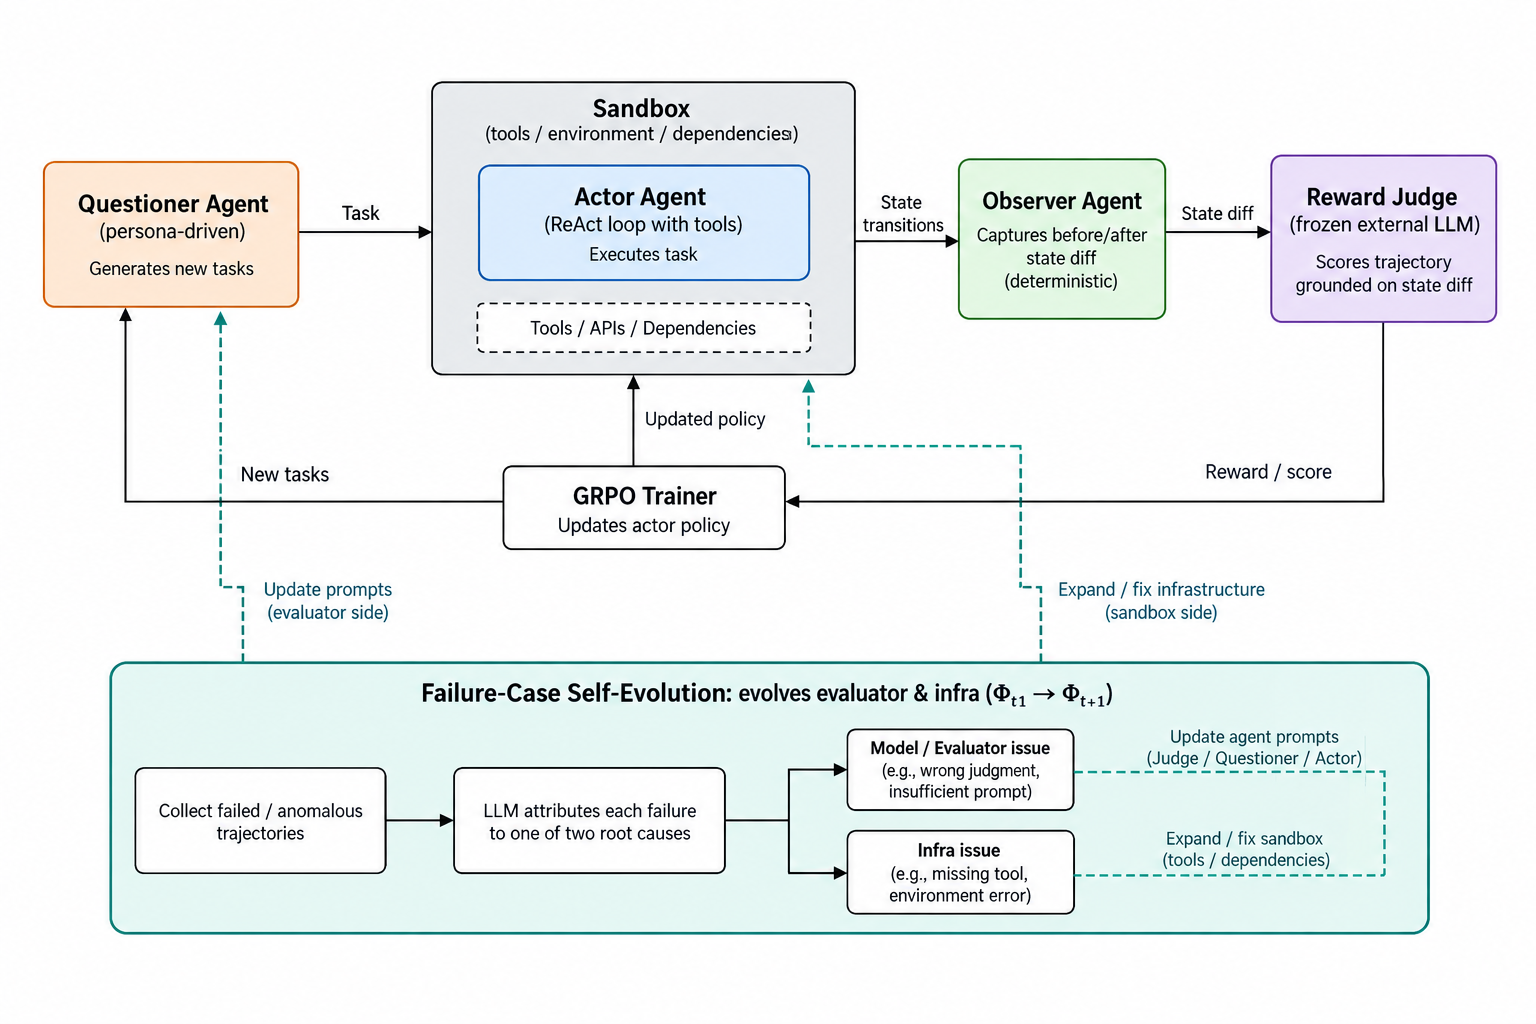
\includegraphics[width=\columnwidth]{arch.png}
\caption{Overall system architecture: three collaborating agents, a code sandbox, a frozen judge, and a GRPO trainer connected through framework injection points.}
\label{fig:arch}
\end{figure}

A self-evolving process is modeled as repeated application of a transition operator $\mathcal{T}$ on the system state $\sigma_t=(\theta_t, s_t, Q_t, \Phi_t)$---policy parameters, sandbox state, task set, and evaluator/infrastructure state, respectively. Within one step, the main loop runs in three stages:
\begin{align}
Q_t &\xrightarrow{\ \pi_{\theta_t}\ } \tau_t \xrightarrow{\ \text{Observer}\ } d_t, \\
d_t &\xrightarrow{\ \text{Judge}(\cdot;\Phi_t)\ } R_t \xrightarrow{\ \text{GRPO}\ } \theta_{t+1}, \\
(\tau_t, d_t) &\xrightarrow{\ \text{Questioner}\ } Q_{t+1}.
\end{align}
Beyond the main loop, the evaluator/infrastructure state $\Phi_t$ evolves at a lower frequency, driven by an accumulated failure-case set $\mathcal{B}_{t'}$. Traditional RL is the degenerate case where $Q_t\!\equiv\!Q_0$, $s_t\!\equiv\!s_0$, $\Phi_t\!\equiv\!\Phi_0$ and only $\theta_t$ evolves; our system evolves all four dimensions.

\section{Method}

\subsection{Cross-Step Self-Evolving Task Generation}

This mechanism lets the system produce every post-seed task without external supply. The core idea is to \emph{grow the next task on the previous step's real execution results}. After each step, for every surviving group the system takes the best trajectory and its sandbox state; an observer optionally summarizes the ``intent--artifact--gap'' of that trajectory; the sandbox file-system state is inherited into a fresh sandbox (true state inheritance, not a textual description); and a persona-driven questioner generates the next seed. Fig.~\ref{fig:selfevolve} illustrates the loop.

\begin{figure}[t]
\centering
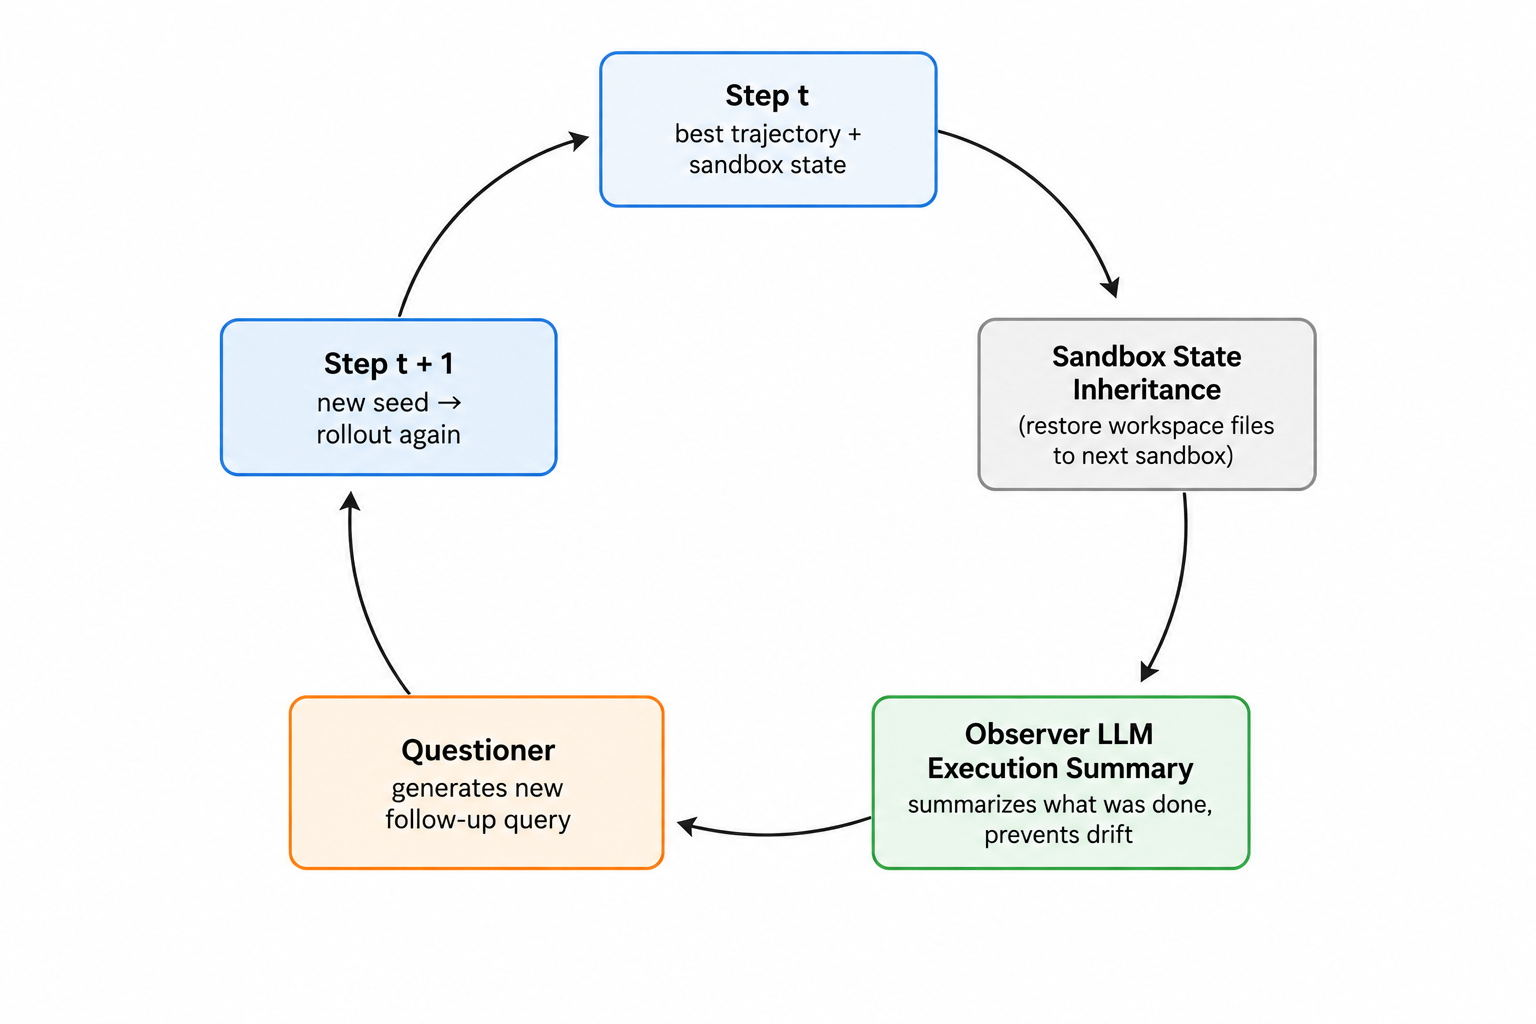
\includegraphics[width=\columnwidth]{selfevolve.png}
\caption{Cross-step self-evolution: the best trajectory's sandbox state is inherited, and a questioner generates the next task from summarized experience.}
\label{fig:selfevolve}
\end{figure}

We make the execution summary \emph{stochastically enabled}, yielding two complementary task modes: a \emph{continuation mode} (summary on) that extends prior work into a long-horizon chain, and a \emph{fresh-task mode} (summary off) that poses a new task on the inherited environment alone. Using a summary rather than the raw trajectory is deliberate: replaying the old policy's verbatim text into the new policy's context would inject off-policy bias and distribution shift; the summary keeps only task-level information stripped of the old policy's generation traces.

\subsection{Multi-Agent Autonomous Data Generation}

A single sampling becomes a complete ``ask--execute--attest'' interaction driven by three agents with separated responsibilities (Fig.~\ref{fig:multiagent}). The \textbf{actor} (the trained policy) solves tasks via ReAct in the sandbox. The \textbf{observer} takes read-only snapshots before and after execution and computes a deterministic state diff; it relies only on environment evidence, never on the actor's self-report. The \textbf{questioner} plays a persona-driven simulated user and generates next-step seeds. Because task solving and follow-up are open-ended generation while attestation must be objective, this ``capability vs.\ determinism'' separation is what makes diff-driven reward trustworthy. From a data-source view, training data emerges from the mutual interplay among these units---a form of self-play grounded in a real sandbox and adjudicated by environment state rather than free text. The use of role-specialized agents to generate interaction data follows the spirit of CAMEL~\cite{camel} and multi-role self-evolution such as R-Zero~\cite{r_zero}.

\begin{figure}[t]
\centering
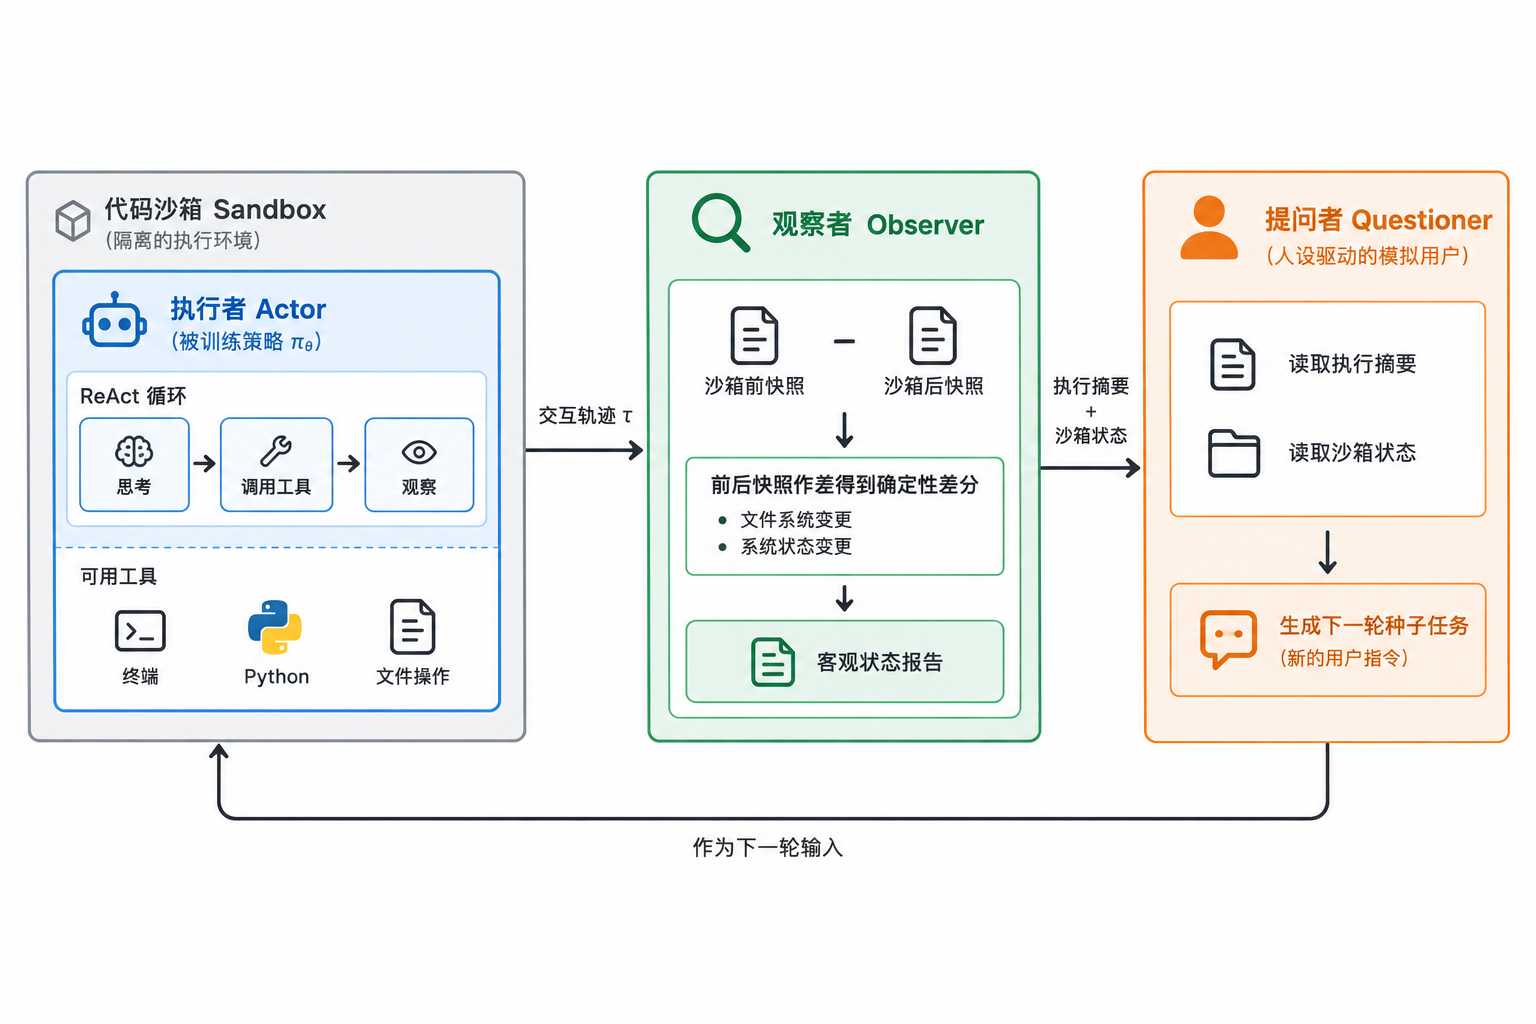
\includegraphics[width=\columnwidth]{multiagent.png}
\caption{Multi-agent collaborative data generation: actor, observer, and questioner chained on one sandbox session.}
\label{fig:multiagent}
\end{figure}

\subsection{Oversample--Eliminate--Select}

To improve per-step signal quality, inference and training are decoupled. Each step oversamples $S$ seeds $\times\,n$ rollouts; groups whose maximum reward is both in the bottom 20\% \emph{and} below a threshold are eliminated (at least 80\% retained); the surviving $R$ groups are ranked by mean absolute intra-group advantage, and the top $N$ groups enter GRPO. This ``dynamic sampling, filter invalid groups'' idea is in line with DAPO~\cite{dapo}. The rationale: GRPO gradients are driven by intra-group advantage, so zero-variance (all-pass/all-fail) groups contribute no effective update. Selecting the highest-signal subset maximizes expected policy improvement under a fixed training budget.

\subsection{Diff-Driven Reward}

The reward's evidence base is shifted from ``what the agent says'' to ``what actually happened in the environment.'' A frozen judge scores from the observer's deterministic state diff (file-system and system-state changes); the actor's self-report is used only for cross-checking. Scoring is multiplicative over multiple dimensions (task completion, correctness, trajectory quality), so a zero on any key dimension yields zero overall; a safety dimension is a binary gate. If the diff is empty (no environment effect), the system short-circuits to zero without calling the judge. Formally, for any behavior change $\delta$ that alters only the self-report but not the state diff ($d(\delta)=d$), we have $\mathbb{E}[R\mid\delta]=\mathbb{E}[R]$: pure verbal hacking is fully blocked, and any reward increase requires a real change in the environment.

\subsection{Failure-Case-Driven Self-Evolution of Evaluator and Infrastructure}

Beyond tasks and policy, a complete self-evolving agent should evolve its \emph{evaluator} (scoring/questioning prompts) and \emph{infrastructure} (tools, sandbox, execution environment). Prior work shows failures can be attributed and repaired via verbal reflection~\cite{reflexion} and that missing capabilities can be distilled into a reusable skill library~\cite{voyager}. Building on this, the system periodically collects failure cases (execution failures, reward anomalies, claim--diff contradictions). Every 10 steps or once 20 cases accumulate, an LLM attributes each case to the \emph{model side} (policy planning, tool use, or plan selection) or the \emph{infrastructure side} (missing dependency, missing tool, short timeout, harness defect). Model-side failures trigger incremental prompt revisions; infrastructure-side failures trigger tooling expansion or distillation of missing capabilities into reusable skills.

\subsection{Self-Evolution Stability Control}

Running unattended, the system monitors five collapse indicators on the existing compute path: reward std, advantage std, policy KL, training loss (NaN/Inf), and surviving-group count. Any single trigger terminates training, since each corresponds to a distinct failure mode under which further steps would only waste compute.

\section{Experiments}

\subsection{Setup}

The base model is Qwen3.5-9B with standard GRPO; inference and training are asynchronously decoupled. Formal training uses 2 nodes $\times$ 8 H800 GPUs, $N{=}64$ groups per step, running 50 steps (manually stopped for comparability with conventional RL; the system itself imposes no step cap beyond the stability criterion). All results below come from \emph{one} end-to-end run, observed along different dimensions.

\subsection{Self-Sustaining Loop and Reward}

The oversample amount $S$ shrinks monotonically and stabilizes near $N$ without collapsing to zero, and cross-step seed generation succeeds at every step---confirming a self-sustaining loop under no external data supply. Fig.~\ref{fig:reward} compares reward-mean curves of self-generated data against a replay-data baseline under an identical GRPO pipeline. Self-generated data rises steadily from about 0.33 to about 0.55, tracking and slightly exceeding the baseline: its training value is no weaker than real replay data.

\begin{figure}[t]
\centering
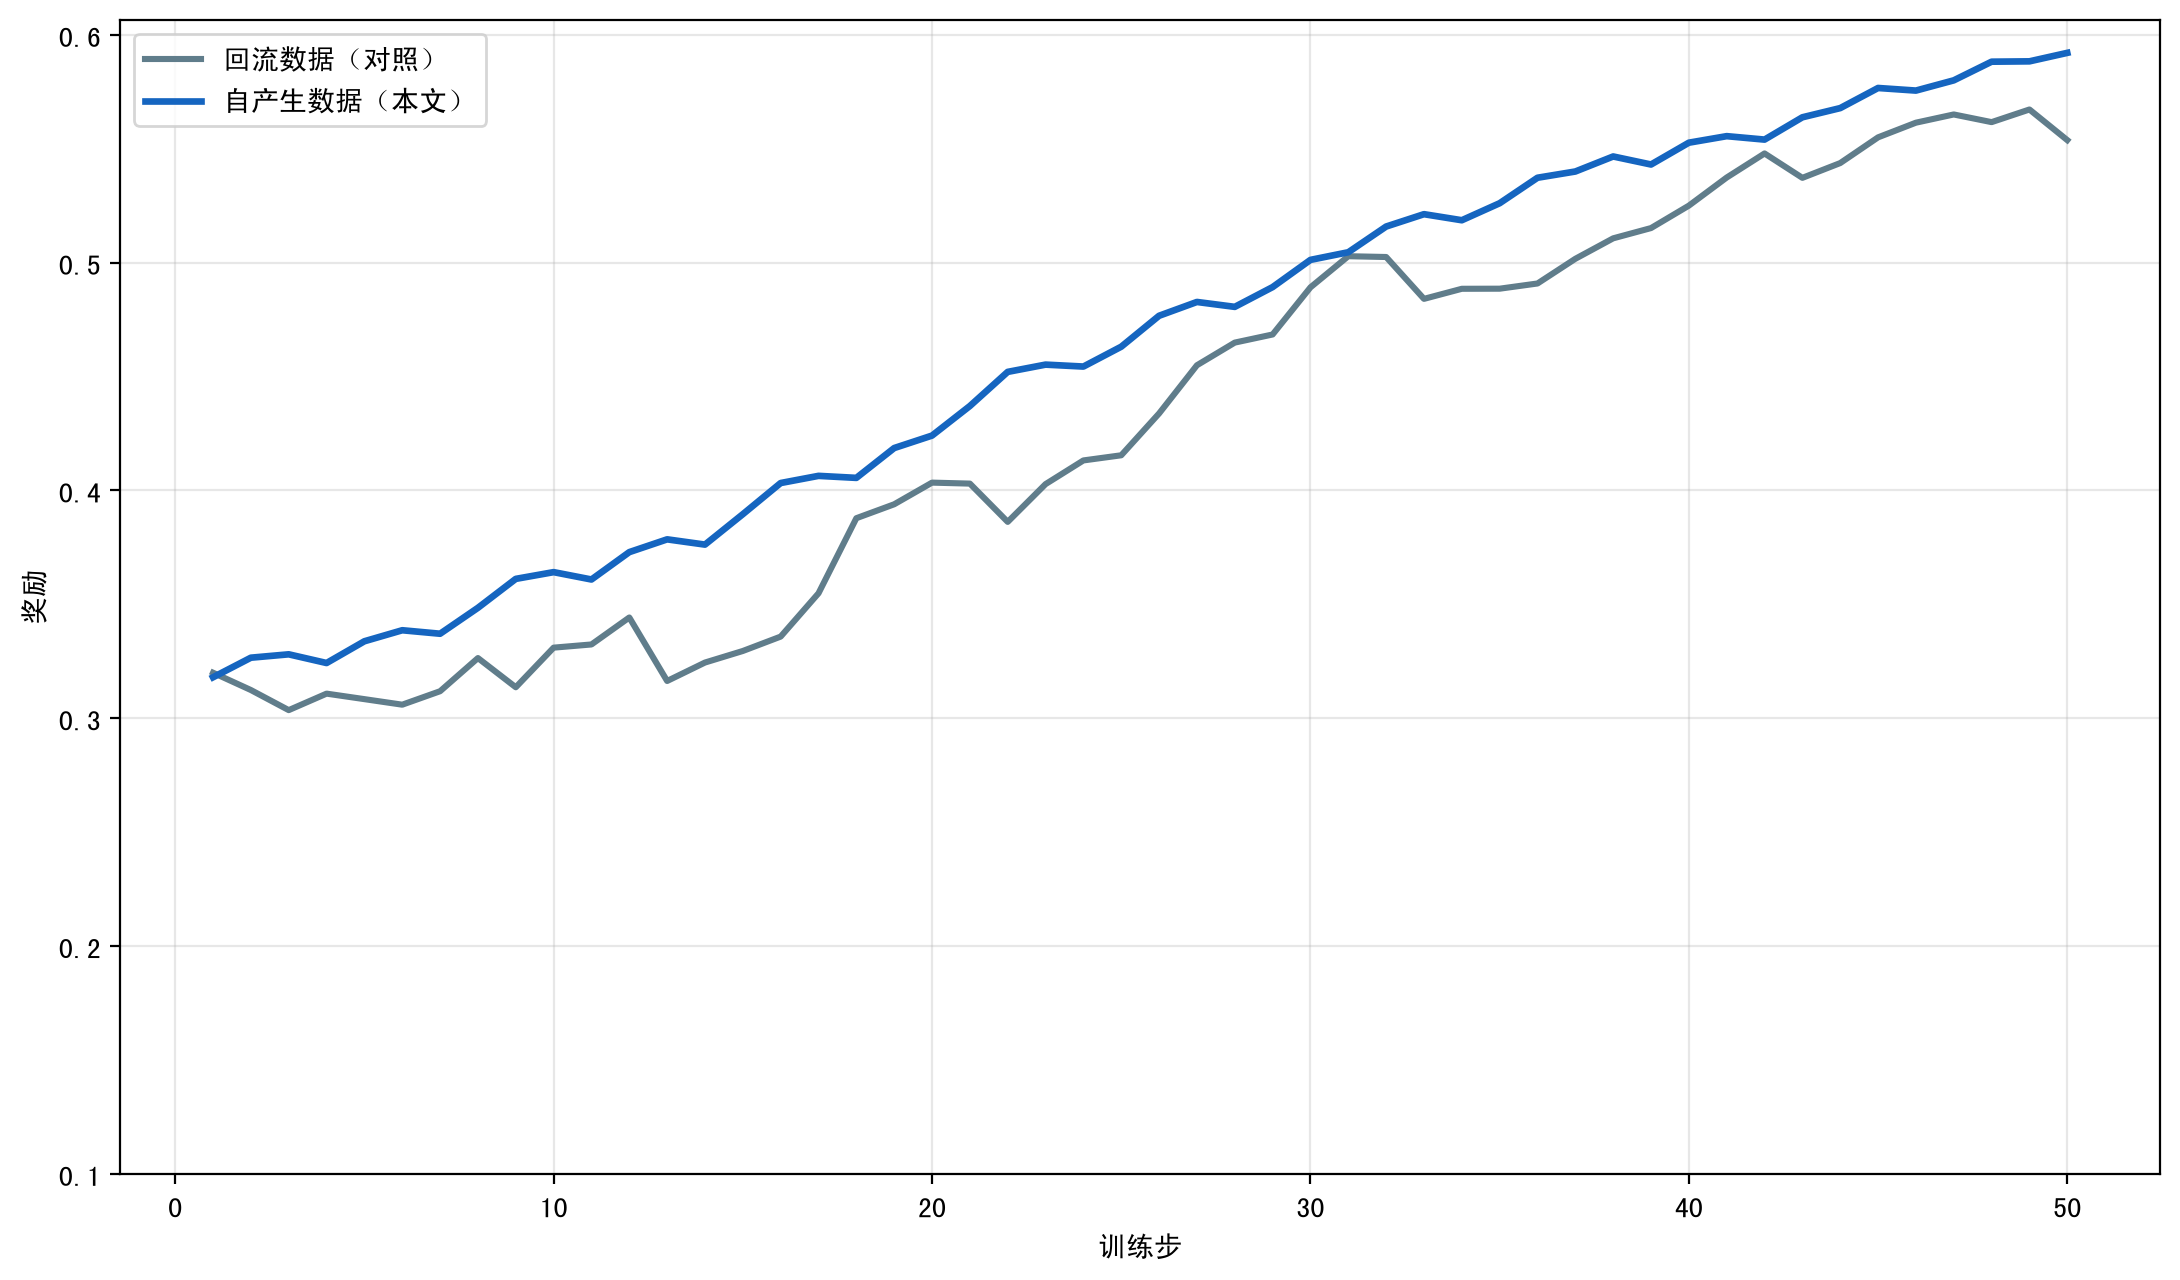
\includegraphics[width=\columnwidth]{reward.png}
\caption{Reward-mean over training steps (EMA-smoothed): self-generated data (ours) vs.\ replay-data baseline.}
\label{fig:reward}
\end{figure}

A companion signal, the intra-group reward std, gradually narrows for self-generated data (a mild variance collapse / Echo-Trap~\cite{echo_trap} precursor) while the baseline stays flat---self-generated data trends toward homogeneity across rounds, whereas externally injected replay data sustains diversity.

\subsection{Capability Evaluation}

Process metrics alone cannot prove a genuine capability gain: since the reward scale itself evolves, higher reward may merely reflect the system inflating its own score. We therefore use an offline benchmark (ClawEval text tasks) as a ruler \emph{independent} of the training loop, comparing three models: the untrained base, a replay-data-trained model, and our self-evolution-trained model. As shown in Fig.~\ref{fig:eval}, our model scores 0.401, clearly above the untrained base (0.370); because this evaluation is independent of the training reward, the gain reflects a real improvement in capability rather than inflated training metrics. Generation diversity drops slightly (0.285 vs.\ 0.294 for base), consistent with the variance collapse observed during training, so process and endpoint metrics agree.

\begin{figure}[t]
\centering
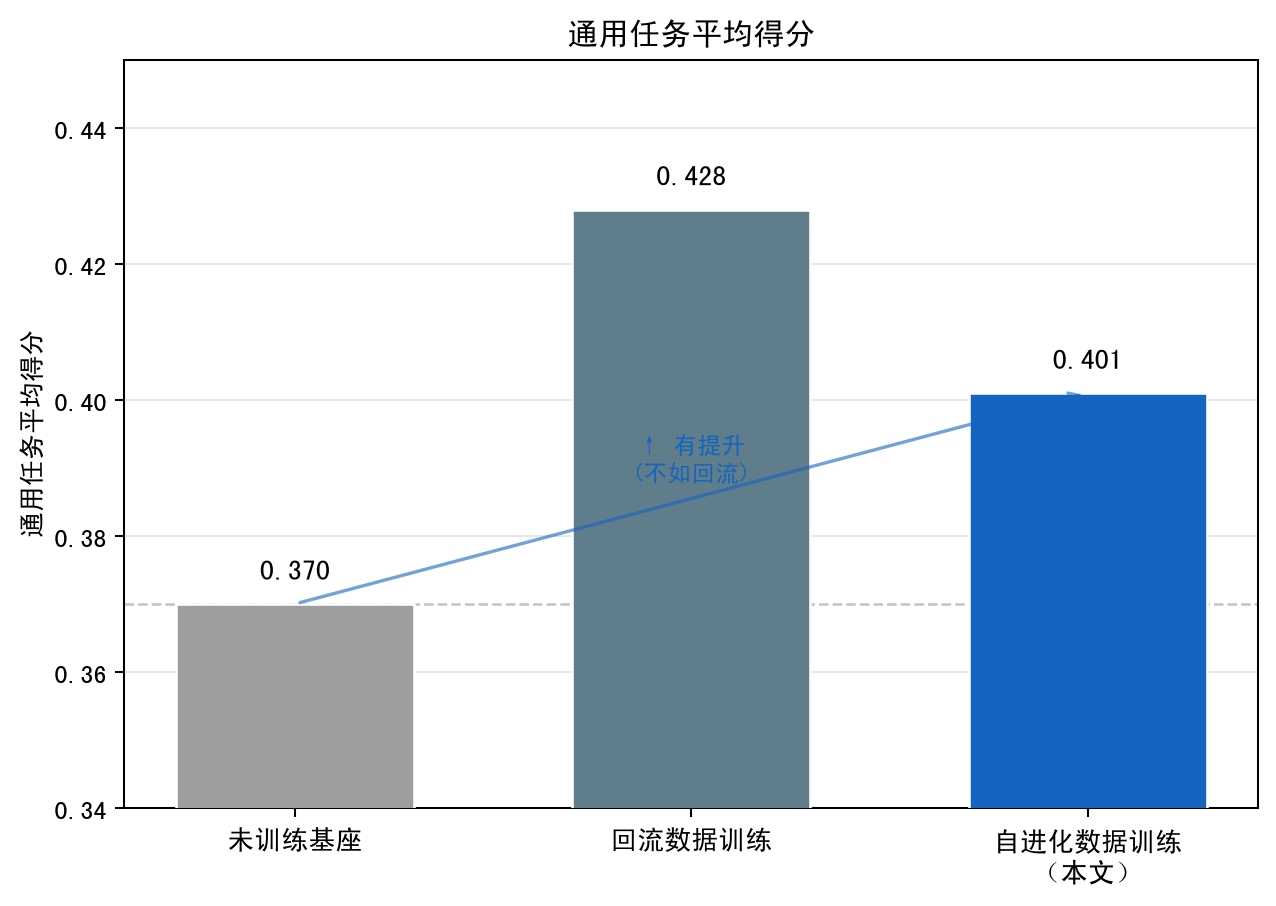
\includegraphics[width=0.8\columnwidth]{eval_score.png}
\caption{Average score on general tasks for the three models; the offline benchmark is independent of the training reward.}
\label{fig:eval}
\end{figure}

\section{Conclusion}

We presented a self-evolving RL system for agentic LLMs that spans both the model level and the agent level, extending the object of self-evolution from ``policy'' alone to ``task, policy, evaluator, and infrastructure.'' The system autonomously generates data, anchors rewards on deterministic environment state diffs, filters trajectories for gradient quality, and evolves its evaluator and tooling from failure cases. End-to-end on Qwen3.5-9B, a small seed set drives complete RL training with no external data, and an independent benchmark confirms a real capability gain over the untrained base model. Multi-modal extension, diversity regularization, and larger-scale training are natural next directions.

\begin{thebibliography}{00}
\bibitem{self_evolution_survey} Z. Tao \emph{et al.}, ``A survey on self-evolution of large language models,'' arXiv:2404.14387, 2024.
\bibitem{self_improve} J. Huang \emph{et al.}, ``Large language models can self-improve,'' arXiv:2210.11610, 2022.
\bibitem{self_play} Z. Chen \emph{et al.}, ``Self-play fine-tuning converts weak language models to strong language models,'' arXiv:2401.01335, 2024.
\bibitem{self_rewarding} W. Yuan \emph{et al.}, ``Self-rewarding language models,'' arXiv:2401.10020, 2024.
\bibitem{rlaif} H. Lee \emph{et al.}, ``RLAIF: Scaling reinforcement learning from human feedback with AI feedback,'' arXiv:2309.00267, 2023.
\bibitem{absolute_zero} A. Zhao \emph{et al.}, ``Absolute Zero: Reinforced self-play reasoning with zero data,'' arXiv:2505.03335, 2025.
\bibitem{reward_hacking_def} J. Skalse \emph{et al.}, ``Defining and characterizing reward hacking,'' in \emph{NeurIPS}, 2022.
\bibitem{reward_overoptimization} L. Gao, J. Schulman, and J. Hilton, ``Scaling laws for reward model overoptimization,'' arXiv:2210.10760, 2022.
\bibitem{grpo} Z. Shao \emph{et al.}, ``DeepSeekMath: Pushing the limits of mathematical reasoning in open language models,'' arXiv:2402.03300, 2024.
\bibitem{react} S. Yao \emph{et al.}, ``ReAct: Synergizing reasoning and acting in language models,'' arXiv:2210.03629, 2022.
\bibitem{codeact} X. Wang \emph{et al.}, ``Executable code actions elicit better LLM agents,'' arXiv:2402.01030, 2024.
\bibitem{dapo} Q. Yu \emph{et al.}, ``DAPO: An open-source LLM reinforcement learning system at scale,'' arXiv:2503.14476, 2025.
\bibitem{echo_trap} Z. Wang \emph{et al.}, ``RAGEN: Understanding self-evolution in LLM agents via multi-turn reinforcement learning,'' arXiv:2504.20073, 2025.
\bibitem{camel} G. Li \emph{et al.}, ``CAMEL: Communicative agents for `mind' exploration of large language model society,'' arXiv:2303.17760, 2023.
\bibitem{llm_judge} L. Zheng \emph{et al.}, ``Judging LLM-as-a-judge with MT-Bench and Chatbot Arena,'' arXiv:2306.05685, 2023.
\bibitem{r_zero} C. Huang \emph{et al.}, ``R-Zero: Self-evolving reasoning LLM from zero data,'' arXiv:2508.05004, 2025.
\bibitem{voyager} G. Wang \emph{et al.}, ``Voyager: An open-ended embodied agent with large language models,'' arXiv:2305.16291, 2023.
\bibitem{reflexion} N. Shinn \emph{et al.}, ``Reflexion: Language agents with verbal reinforcement learning,'' arXiv:2303.11366, 2023.
\end{thebibliography}

\end{document}
